\documentclass[11pt]{article}
\usepackage{geometry}                % See geometry.pdf to learn the layout
\usepackage{graphicx}
\usepackage{amssymb}
\usepackage{epstopdf}

\title{Compte-rendu du TEA n°3}
\author{\textsc{Valentin GAUTHIER}\\ Alexandre TORRES--LEGUET}

\begin{document}
\maketitle

\section{Introduction}
%présentation du problème, le contexte

\quad \quad Ce compte-rendu présente le travail réalisé dans le cadre du TEA 3 de l'enseignement d'AAP, qui se concentre sur le tri rapide et le tri fusion en \textsc{C}.
 
Nous avons vu en TD le principe de fonctionnement et le code de ces tris en \textsc{C}, notre tâche a alors été dans un premier temps d'adapter ce travail afin de le rendre compatible avec les outils de création de graphiques, i.e. avec la structure de données \texttt{T\textunderscore data}. 

Dans un second temps, nous avons implémenté les fonctions \texttt{fusionsort} et \texttt{quicksort} qui respectent le même prototype que la fonction \texttt{qsort} disponible nativement dans \textsc{C}. (sous réserve d'inclure \texttt{stdlib.h})

Enfin, nous avons implémenter le tri fusion sur des listes chaînées.



\section{Développement}
%organisation du programme
%organisation du groupe (qui a fait quoi)
%difficultés

\subsection{Tri fusion}

\quad \quad Le dossier \texttt{tri\textunderscore fusion} recense notre travail relatif au tri fusion sur un tableau. \\

Pour cette partie, la première partie du travail a été de transformer la fonction d'en-tête

$$
\texttt{void tri\textunderscore fusion(T\textunderscore elt t [], int debut, int fin)}
$$

en la fonction

$$
\texttt{void tri\textunderscore fusion(T\textunderscore data d, int n)}
$$

où \texttt{n} désigne le nombre d'éléments à considérer à partir du début du tableau passé. Il faut donc, au moment d'appeler cette deuxième fonction, envoyer la bonne partie du tableau (et non pas le tableau entier comme c'est le cas pour la première fonction). \\

Nous avons effectué ensemble la fonction \texttt{fusionsort} une fois la fonction \texttt{quicksort} implémentée car cette dernière nous a paru plus abordable pour gérer le type \texttt{void *} que l'on récupère en entrée.

\subsection{Tri rapide}

\quad \quad Le dossier \texttt{tri\textunderscore rapide} recense notre travail relatif au tri fusion sur un tableau. \\

Le même travail de conversion a été effectué afin de rendre compatible la fonction vue en TD au type \texttt{T\textunderscore data}. \\


La fonction \texttt{quicksort} reprend les mêmes idées que \texttt{tri\textunderscore rapide}. Cependant, l'implémentation concrète du tri a été amené à changer. La plus grosse difficulté rencontré a été que le tableau passé en entrée est de type \texttt{void *} (i.e. type non déterminé).
Cela a notamment posé un problème dans la fonction annexe \texttt{echanger} qui a pour but d'échanger 2 éléments d'un tableau. En effet, le compilateur nous empêche d'assigner une valeur à type \texttt{void *} : la solution pour pallier à cela a été d'utiliser la fonction native \texttt{memcpy} afin de ne pas avoir à assigner une valeur. 

\subsection{Tri rapide sur une liste chaînée}

\quad \quad Le dossier \texttt{tri\textunderscore fusion\textunderscore listes} recense notre travail relatif au tri fusion sur une liste chaînée.

Nous nous sommes d'abord concentré sur la fonction \texttt{split}, qui a pour but de diviser en 2 moitié une liste chaînée. Cette fonction, au lieu de retourner 2 valeurs qui sont les têtes des 2 listes, modifie 2 pointeurs (\texttt{T\textunderscore node **front} et \texttt{T\textunderscore node **back}) qui, une fois la fonction terminée, pointeront sur les 2 listes divisées.

Voici un schéma explicatif qui montre le déroulement de cette division : 

\begin{center}
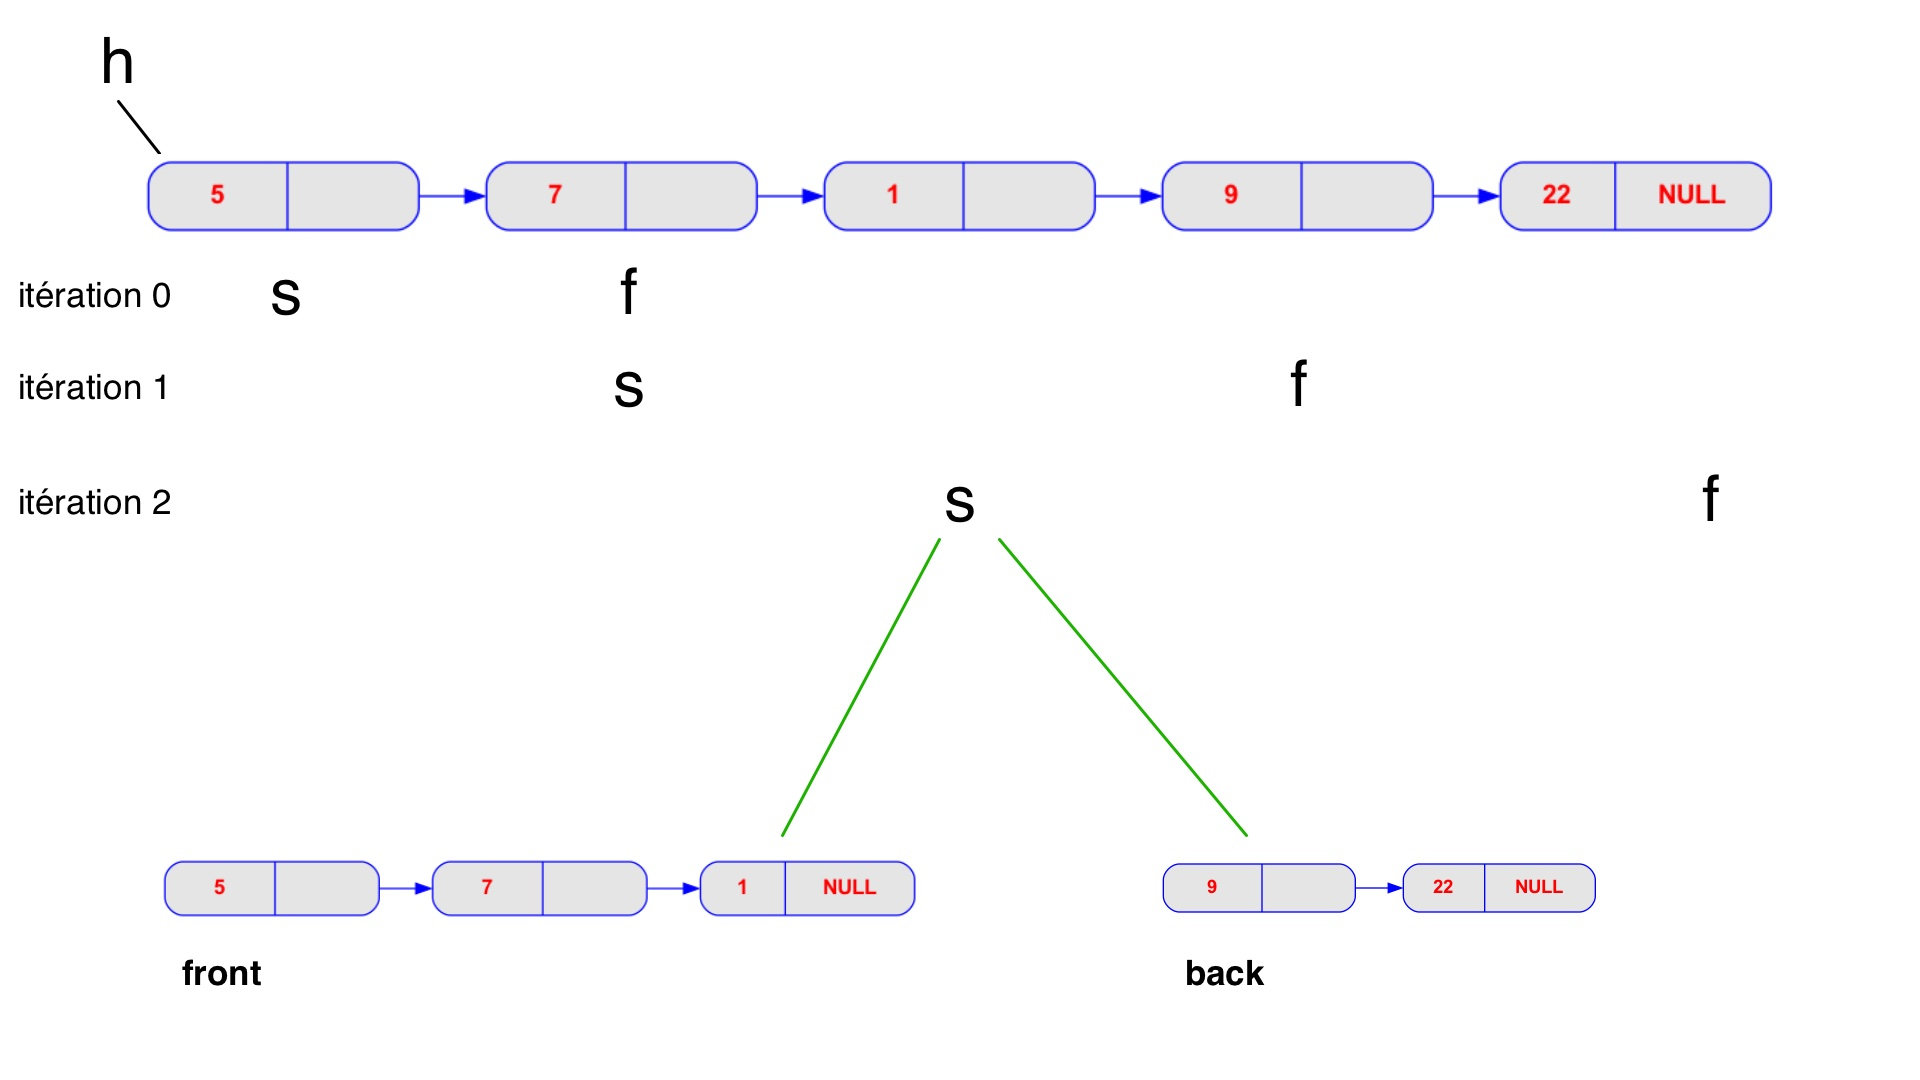
\includegraphics[scale=0.25]{images/2.jpg}
\end{center}

\texttt{s} et \texttt{f} correspondent aux variables \texttt{slow} et \texttt{fast} de notre code : ces pointeurs parcourent la liste, mais un le fait de manière "lente" (une maille à la fois) et l'autre le fait plus rapidement (deux mailles à la fois). Il s'en suit que, lorsqu'on les fait parcourir la liste, à la fin, lorsque \texttt{f} atteint le bout de la liste, \texttt{s} se trouve au milieu de la liste. On s'en sert alors pour découper la liste en deux. \\


La fonction \texttt{merge} fusionne 2 listes chaînées supposées triées. Le principe est le même qu'avec le tableau : on compare les premiers éléments de chacun des deux listes à fusionner, on sélectionne le petit, puis on recommence... jusqu'à épuisement des deux listes. \\

La fonction \texttt{merge\textunderscore sort} se tâche simplement de diviser la liste d'entrée, trier récursivement les deux listes obtenues, et de les fusionner. \\

Voici un schéma permettant d'illustrer le tri fusion sur une liste chaînée :

\begin{center}
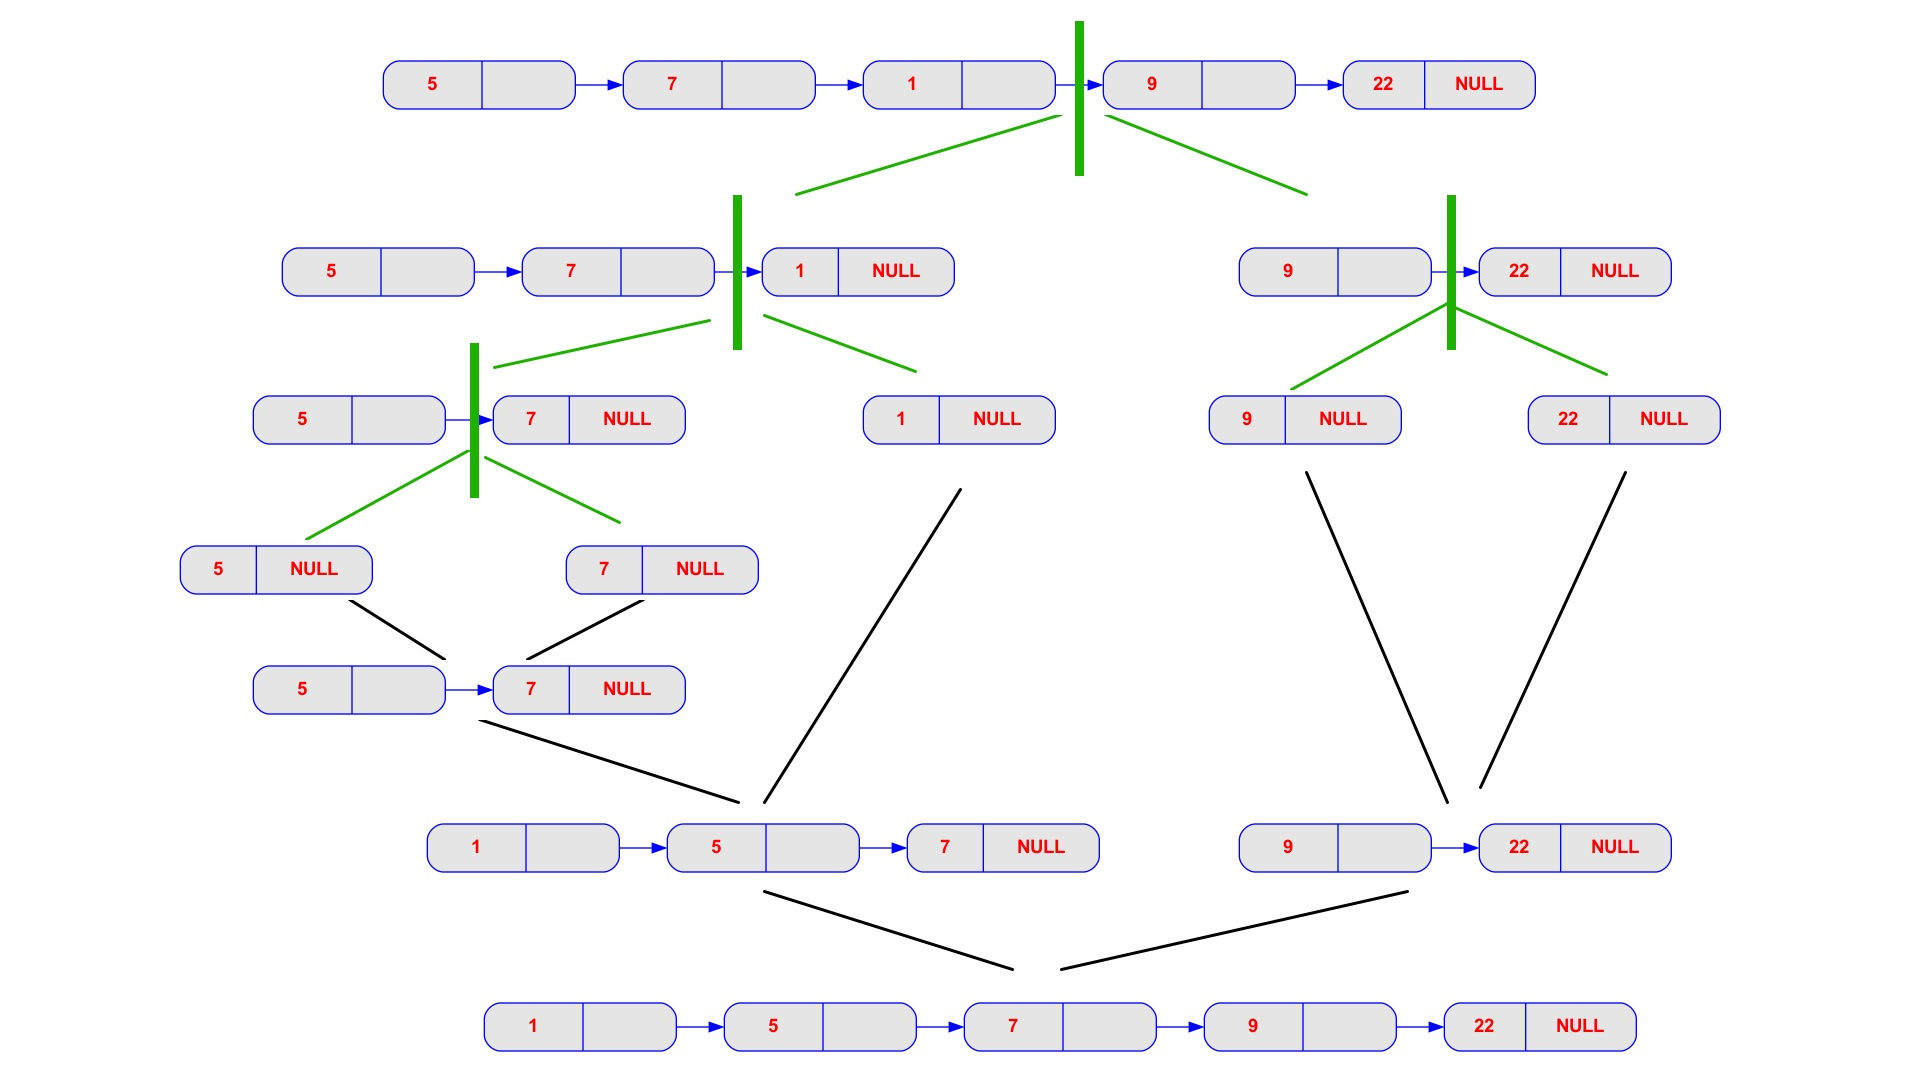
\includegraphics[scale=0.25]{images/1.jpg}
\end{center}

\subsection{Organisation - Gestion de projet}

Concernant l'organisation des tâches au sein du groupe, Valentin s'est chargé de la partie concernant le tri fusion et Alexandre celle du tri rapide. Ce travail a été opéré le week-end qui a suivi notre séance de TP du vendredi.

Enfin, au cours du début de la semaine suivante, nous avons pu nous réunir afin de réfléchir à adapter et implémenter l'algorithme de tri fusion sur une liste chaînée. Pour cela, nous sommes revenus sur la séance de TP antécédente pendant laquelle nous avions implémenté le type de liste chaînée (fichiers \texttt{list.h} et \texttt{list.c}).




\section{Résultats}
%présentation des résultats, jeux d'essais, analyse, temps d'exec...

Voici, pour 2 jeux d'essais, les temps d'exécutions constatés sur l'une de nos machines (par moyenne).
Le premier exemple correspond à une cible parfaite, tandis que le second ne peut qu'être approché, d'où la longueur de l'exécution.

\begin{center}
\begin{tabular}{||c c c||} 
 \hline
 cartons & cible & temps \\ [0.5ex] 
 \hline\hline
 3 5 7 9 25 50 & 788 & 1.2s \\ 
 \hline
 2 2 3 4 6 10 & 631 & 23.6s \\ [1ex] 
\hline
\end{tabular}
\end{center}

Il est intéressant de remarquer que ces temps d'exécutions sont bien meilleurs que ceux constatés avec notre implémentation \textsc{Python}.

\section{Schéma d'exploration}

Notre algorithme, étant donné un RPN, cherche à lui ajouter un à un tous les opérateurs, puis un à un les cartons restants.
Une amélioration que nous avons effectué est que, si jamais un RPN peut être évalué sous forme d'une valeur (exemple : $1 \; 2 \; +$ qui peut être évalué à $3$) alors lui ajouter un opérateur le rendra nécessairement invalide. Sur le schéma, on voit que cette amélioration évite l'exploration inutile d'un grand nombre de noeuds de l'arbre.


\section{Conclusion}
%analyser les problèmes, perspectives

\quad \quad Au terme du travail, il vient que notre programme semble fonctionner grâce à plusieurs tests tous réalisés avec justesse. Nous restons conscients que c'est un algorithme de type "glouton".

\end{document}  
